\chapter{Control Methods for Nonlinear Systems}
    The boiler system is inherently nonlinear so that an adequate control method must be implemented for its safe and efficient operation.
    Common industry practice in this respect is to implement the three-element control, which is fundamentally the PID control structure which is first discussed. Then we also present the linear quadratic control (LRQ) which is a powerful control method used in many industrial applications, which however has its limitations when applied to nonlinear systems. In fact, both PID and LQR control methods cannot be used for nonlinear systems unless the system model is linearized. As is well known, the linearized model is valid only if the process operates in a small neighborhood with respect to the nominal operating state. For large variations in the operating state, it is necessary that a nonlinear control method be utilized. The Model Predictive Control (MPC) is one of the powerful, yet simple, methods for controlling nonlinear systems, and has attracted the attention of engineers in the profession. This chapter introduces the fundamentals of the MPC control method, which will be used in this thesis for controlling the steam boiler.

    \section{Three Element Level Control}
        Three Element Control refers to the number of measurements or Process Variables (PV) that are used in the control calculation. These measured elements are:
        
        \begin{itemize}
          \item $l$ - Liquid Level in the Drum
          \item $q_f$ - Feed-water Flow into the Drum
          \item $q_s$ - Steam Flow leaving the Drum 
        \end{itemize}
        
        \begin{figure}[ht]
            \begin{center}
                \resizebox{\ScalePIDControlImageA \textwidth}{!}{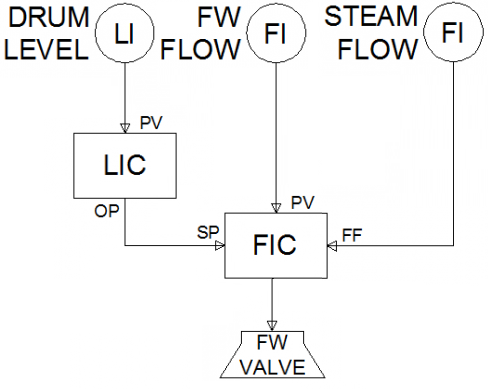
\includegraphics{Graphics/Three_Element}}
                \caption{Three Element Control \cite{crossco}}
                \label{fig:3_element_control}
            \end{center}
        \end{figure} 
        
        Three Element Control \cite{crossco} consists of two PI(D) loops in cascade control, and a feed forward control. This can be seen in Figure \ref{fig:3_element_control}. The two loops in cascade are a fast acting internal loop for feed-water and a slower external loop for drum level. In a cascade control scenario, the external loop's output (OP) is used as the Set Point (SP) for the inner loop. 
        The feed forward (FF) of steam flow is applied to the internal loop. An alternative, and less popular configuration can have the feed forward on the outer loop, as seen in Figure \ref{fig:Alt_3_element_control}. It should be noted that a cascaded control setup has several drawbacks, including integral windup due to the inner loop being at a physical limit but the outer loop still attempting to control. 
        %{\bf Give a better description of the two figures on three element control.  There are many symbols that are not defined.} % Biswas Notes % % Robs Notes - Should be fixed in above paragraph %

        \begin{figure}[ht]
            \begin{center}
                \resizebox{\ScalePIDControlImageB \textwidth}{!}{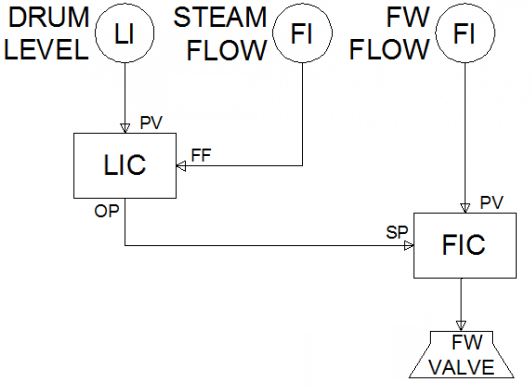
\includegraphics{Graphics/Three_Element_2}}
                \caption{Alternative Three Element Control \cite{crossco}}
                \label{fig:Alt_3_element_control}
            \end{center}
        \end{figure}



        %{\bf Add a paragraph on {\it shrink and swell} effect here}.   %% BISWAS NOTES %%
        %Shrink and swell refers to a phenomenon that when the drum pressure drops, some water in the tubes flashes, and those steam bubbles push water in the tubes above them up into the drum, temporarily raising the drum level. Then when the system stabilizes and those steam bubbles either collapse or reach the drum, the tubes rapidly refill with water from the drum, dropping its level. The effect is asymmetrical - when drum pressure rises due to falling steam demand, it temporarily suppresses the production of steam in the tubes but the effect is more subtle. \cite{crossco} 
        % Rob Notes - Moved to chapter 1 %
        
        Single Element and Two Element control are used at lower feed-water flows or lower load, where the shrink and swell effects are not as prevalent. Single Element control is a PI(D) Level control loop, and Two Element control is the same as Three Element control, without the feed forward.
        
        %The cascade control must be tuned with the following procedure. The outer loop is switched to manual mode and the inner loop is tuned, then, the inner loop is placed in automatic control mode and the outer loop is tuned.
        
        In this control mode, Throttle Pressure is usually controlled by a simple PI(D) loop. Total power output may be controlled instead of throttle pressure. The turbine is often modeled as a first order system with the input of Throttle Pressure and the output of mechanical power \cite{controlguruWebsite}.

        \subsection{Application in Boiler Controls}

        By design, the PID control is used to minimize error with respect to a desired operating reference using specific tuning parameters. It does not allow any optimization of the process operation, such as minimization of fuel consumption (or control energy), nor does it account for any boundary conditions. Industry experts also use adaptive tuning controllers due to the fact that the tuning parameters can vary with load. Optimization of process operation could be achieved using optimal  and robust control methods as presented next.

    \section{Linear Quadratic Regulator}
    
        The Linear Quadratic Regulator (LQR) is one of powerful methods for optimizing the process operation.  In this method, the system performance is defined in terms of a cost function which is a measure of cost of state error and cost of control.  The objective is to find a control that minimizes the cost function.  For a discrete time linear system,
        
        \begin{equation} 
            \label{eq:lqr1}
            x(k+1) = A x(k) + B u(k)
        \end{equation}
        
        where $x_k$ is the state vector and $u_k$ is the control vector, and the state and control matrices $A$ and $B$ are of compatible dimension.  The cost function is taken as
        
        \begin{equation}
            \label{eq:lqr2}
            J = \sum_{0}^{\infty} \left ( x_k^T Q x_k + u_k^T R u_k\right )
        \end{equation}
        
        where $Q$ is a positive semidefinite matrix and $R$ is a positive definite matrix.
        Here the first term of the cost function represents the cost due to state error with respect to the reference (which is taken as zero in this case), and the cost of control.
        The optimal control sequence that minimizes the cost function is given by the discrete time Riccati equation
        
        \begin{equation}
            \label{eq:lqr3}
            \aligned
                P &= A^TPA - (A^TPB)(R+B^TPB)^{-1}(B^TPA)+Q\\
                K_{lqr} & = (R+B^TPB^{-1})(B^TPA)\\
                u_k & = K_{lqr} x_k
            \endaligned
        \end{equation}
        
        By solving the Riccati equation, one obtains the matrix $P$ which is a positive symmetric definite matrix, which is then used to find the feedback gain $K_{lqr}$ for the control loop.  In this method, the Riccati matrix $P$ can be computed before the control loop initiates.  From the design perspective, one must choose the appropriate weighting matrices $Q$ and $R$ matrices so as to obtain the desired closed loop performance.
        
        It is important to note that the linear quadratic regulator as discussed above applies to linear systems only.  However there are many practical systems, including the steam boiler discussed in the thesis, are described by nonlinear system model.  For nonlinear systems, one can linearize the system model and then apply the LQR theory.  However the drawback is that this approach works well only when the actual nonlinear system operates within a small neighborhood of the operating point.  For large variations of the system state, the results are usually not acceptable.
        
        %Linear Quadratic Regulators in both the Continuous and Discrete form are solved using different forms of the Riccati Equation. This is useful for Linear systems, as in the name of the control methodology itself describes the type of system it is used in. The Quadratic portion of the name refers to the cost function. Traditional LQR applications in a nonlinear system would see the system being linearized around a point, and providing designing the regulator around that point.
        
        There is some research in applying LQR methodologies to nonlinear systems using the State-Dependent Riccati Equation \cite{Korayem}.  In this method, the one derives  the Riccati equation in which the system model matrices is actually dependent on the current system state.  So fundamentally, this means that the Riccati equation must be solved in real time for each sampling time before the control input is computed. This is not a trivial job as it takes significant computing resources to solve the Riccati differential equations.
        
        % https://math.stackexchange.com/questions/2558102/lqr-controller-for-a-nonlinear-system-how-to-split-the-ss-model-as-a-and-b-mat
        % https://ac-els-cdn-com.libproxy.temple.edu/S0019057814001268/1-s2.0-S0019057814001268-main.pdf?_tid=fe049522-ada0-4187-ad8b-4411fe3bf75d&acdnat=1539568348_aa431eef8ff6d9743feeae876ede3752
        
    \section{Model Predictive Control}
    
        Model predictive control (MPC) \cite{Wang} is a popular control method that has found many applications in chemical industries. MPC is an advanced control method that optimizes the current state satisfying process constraints while at the same time using predicted information of system state in future time slots.
        MPC control strategies are characterized by a explicitly and separately identifiable model of the controlled system. This model is used to calculate the behavior of the plant with the future control signal as adjustable variables.
        
        MPC has direct links to the classical linear quadratic regulator (LQR) in continuous time and discrete time when using a long prediction horizon. The key difference between MPC and LQR is that the MPC solves the optimization problem using a moving time horizon window and optimized along the entire time horizon, while LQR solves the same problem within a fixed window and solves for a single optimal solution.
    
        \subsection{Discrete Time MPC Theory}

            The MPC control method is a receding horizon control method in which one first finds the optimal solution for a predicted time horizon, but apply the control for only one time step.  The process is then repeated for future time slots.
            Consider the linear system in discrete time
            \begin{equation}
                \label{eq:mpc1}
                \aligned 
                    x(k+1) & = A x(k) + B u(k)\\
                    y(k) & = C x(k)
                \endaligned
            \end{equation}
            Denote the control signals for the entire control horizon starting from time slot $k_i$ as
            \begin{equation}
                \label{eq:Trajectory1}
                U(k_i) = \{u(k_i), u(k_i+1), ... , u(k_i+N_c+1)\}
            \end{equation}
            where $N_c$ is the Control Horizon. Then future system States can be denoted as:
            
            \begin{equation}
                \label{eq:mpc2}
                \aligned
                    x(k_i+1|k_i)  =& Ax(k_i) + B u(k_i)\\
                    x(k_i+2|k_i)  =& Ax(k_i+1|k_i) + B u(k_i+1)\\
                                  =& A^{2}x(k_i) + AB u(k_i) + B u(k_i+1)\\
                    x(k_i+3|k_i)  =& Ax(k_i+2|k_i) + B u(k_2+1)\\
                                  =& A^{3}x(k_i) + A^2B u(k_i)+ AB u(k_i+1) + B u(k_i+2)\\
                    x(k_i+N_p|k_i)=& A^{N_p} x(k_i) + A^{N_{p}-1} B u(k_i+1-1) + \cdots\\
                                   & \cdots + A^{N_{p}-N_{c}} B u(k_i+N_c-1)
                \endaligned
            \end{equation}                

            where $N_p$ is the Prediction Horizon. 
            
            Using the above equation, future Controlled Outputs can be computed as:
            \begin{equation}
                \aligned
                    y(k_i)        =& Cx(k_i)\\
                    y(k_i+1|k_i)  =& CAx(k_i) + CB u(k_i)\\
                    y(k_i+2|k_i)  =& CA^{2}x(k_i) + CAB u(k_i) + CB  u(k_i+1)\\
                    y(k_i+3|k_i)  =& CA^{3}x(k_i) + CA^2B u(k_i)+ CAB u(k_i+1) + CB u(k_i+2)\\
                    y(k_i+N_p|k_i)=& CA^{N_p} x(k_i) + CA^{N_{p}-1} B u(k_i+1-1) + \cdots\\
                                   & \cdots + CA^{N_{p}-N_{c}} B u(k_i+N_c-1)
                \endaligned
                \label{eq:outputs1}
            \end{equation}   
            
            The control horizon $N_c$ is chosen to be less than (or equal to) the prediction horizon $N_p$.
            It should be noted that all predicted variables are calculated from the current state, future control movements, and the model information.
            The above equations then can be expressed in matrix form as:
            %{\bf why do you need a control horizon different from prediction horizon?}
            %% Notes Needed Here BISWAS BORZELLIERI %%
            
            \begin{equation}
                \label{eq:Matrix1}
                Y = Fx(k_i) + \Phi U(k_i)
            \end{equation}
            where
            \begin{equation}
                \aligned
                    Y &= \left [ \begin{array}{c} y(k_i+1|k_i) \\ y(k_i+2|k_i)\\\vdots \\ y(k_i+N_{p}|k_i) \end{array}  \right ], \\ \\
                    U &=\left [  \begin{array}{c} u(k_i) \\ u(k_i+1) \\\vdots \\ u(k_i+N_{c}-1) \end{array}  \right ]\\ \\
                    F &= \left [ \begin{array}{c}CA \\ CA^{2}\\\vdots \\ CA^{N_{p}} \end{array}  \right ]\\ \\
                    \Phi &= \left [ \begin{array}{ccccc}
                         CB & 0 & 0 & \cdots & 0 \\
                         CAB & CB & 0 & \cdots & 0 \\
                         CA^{2}B & CAB & CB & \cdots & 0 \\
                         \vdots & \vdots & \vdots & \ddots & \vdots \\
                         CA^{N_{p}-1}B & CA^{N_{p}-2}B & CA^{N_{p}-3}B & \cdots. &  CA^{N_{p}-N_{c}} B \end{array}  \right ]
                \endaligned
            \end{equation}
            
            Suppose the control objective is for the system output $y(k_i)$, $y(k_i+1)$, $\cdots$, $y(k_i+N_p)$ to follow a desired output. Define the set-point desired reference as
            \begin{equation}
                \label{eq:mpc5}
                \aligned
                    R_s &= \overline{R}_s r(k_i)\\
                    \overline R_s^T &= \overset{N_p}{\overbrace{\begin{bmatrix} 1& 1 & ... & 1 \end{bmatrix}}}
                \endaligned
            \end{equation}
            i.e., $\overline R_s$ is the $N_p$-dimensional column vector of ones.
            
            To minimize the tracking error, define the cost function
            \begin{equation}
                \label{eq:Cost1}
                J(U) = \frac12(R_s-Y)^TQ(R_s-Y)+\frac12 U^T R  U
            \end{equation}
            where $Q$ and $R$ are positive definite weighting matrices.  Clearly, the first term minimizes the set-point tracking error and the second term minimizes the cost of control.  The cost function is then minimized subject to the constraint \eqref{eq:Matrix1}.
            
            Substituting equation \eqref{eq:Matrix1} in the above equation, and differentiating with respect to $U$, we obtain
            
            $$\frac{\partial J}{\partial U} = - \Phi^TQ(R_s-Fx(k_i))+(\Phi^{T}Q\Phi + R)U  = 0$$
            which gives the optimal tracking control sequence as
            \begin{equation}
                \label{eq:Optimal1}
                U(k_i) = (\Phi^{T}Q\Phi + R)^{-1}\Phi^{T}Q(R_{s}-Fx(k_i))
            \end{equation}
            
            For closed loop MPC control method, a receding horizon concept is used, and only the first element of the control vector $U$ is used at time slot $k_i$, i.e,
            \begin{equation}
                \label{eq:Control1}
                \aligned
                    u(k_i) &= \overset{N_c}{\overbrace{\begin{bmatrix} I& 0 & ... & 0 \end{bmatrix}}} U(k_i) \\
                           &= \overset{N_c}{\overbrace{\begin{bmatrix} I& 0 & ... & 0 \end{bmatrix}}} (\Phi^{T}Q\Phi + R)^{-1}\Phi^{T} Q( \overline{R}_s r(k_i)-Fx(k_i)) \\
                           &= K_y r(k_i) - K_{mpc} x(k_i)
                \endaligned
            \end{equation}
            where:
            \begin{equation}
                \label{eq:Ky1}
                K_y = \overset{N_c}{\overbrace{\begin{bmatrix} I& 0 & ... & 0 \end{bmatrix}}} (\Phi^{T}Q\Phi + R)^{-1}\Phi^{T} Q\overline{R}_s
            \end{equation}
            \begin{equation}
                \label{eq:Kmpc1}
                K_{mpc} = \overset{N_c}{\overbrace{\begin{bmatrix} I& 0 & ... & 0 \end{bmatrix}}} (\Phi^{T}Q\Phi + R)^{-1}\Phi^{T}Q F
            \end{equation}
            
            Substituting the above control in the system model \eqref{eq:mpc1}, we obtain
            \begin{equation}
                \aligned
                    x(k+1) &= A x(k) + B (K_y r(k_i) - K_{mpc} x(k_i))\\
                           &= (A  - B K_{mpc} )x(k_i) + B K_y r(k_i) \\
                           &= A_{closed}x(k) + B_{closed} r(k_i)
                \endaligned
            \end{equation}
            where
            \begin{equation}
                \aligned
                    A_{closed} &= A - B K_{mpc}\\
                    B_{closed} &= B K_y
                \endaligned
            \end{equation}
            
            The process is then repeated for every time slot in the control horizon.  This completes the MPC control concept for the discrete time linear system.

        \subsection{Discrete Time MPC for Nonlinear Systems}

            The MPC control described above can be extended for nonlinear systems. The basic idea is to linearize the nonlinear system with respect to the current state, and then use the MPC control for one time slot using the method described in the previous section. Then for the next time slot, the nonlinear system is linearized again using the updated system state, which is followed by a new computation of MPC control. The process is continued till the end of desired control horizon.

            Consider the nonlinear system given by
            \begin{equation}
                \label{eq:non1}
                \aligned
                    \dot{x} &= f(x,u) \\
                    y& =g(x,u)
                \endaligned
            \end{equation}
            
            The nonlinear system is then linearized at the current time slot $k_i$ using $\{x(k_i), u(k_i)\}$ to obtain
            
            \begin{equation}
                \label{eq:non2}
                \aligned
                    \frac{\partial\Delta x}{dt}& = A_i^c \Delta x + B_i^c \Delta u\\
                    \Delta y & = C_i^c \Delta x + D_i^c \Delta u
                \endaligned
            \end{equation}
            
            where
            
            \begin{equation}
                \label{eq:non3}
                \aligned
                    A_i^c &= \biggl.\frac{\partial f(x,u)}{\partial x}\biggr|_{x(k_i),u(k_i)}\\
                    B_i^c &= \biggl.\frac{\partial f(x,u)}{\partial u}\biggr|_{x(k_i),u(k_i)}\\
                    C_i^c &= \biggl.\frac{\partial g(x,u)}{\partial x}\biggr|_{x(k_i), u(k_i)}\\
                    D_i^c &= \biggl.\frac{\partial g(x,u)}{\partial u}\biggr|_{x(k_i), u(k_i)}
                \endaligned
            \end{equation}
            
            The above linearized system is then expressed as a discrete time equation as
            
            \begin{equation}
                \label{eq:non4}
                \aligned
                    \Delta x(k_i+1) & = A_i \Delta  x(k_i) + B_i \Delta  u(k_i)\\
                    \Delta y(k_i)   & = C_i \Delta x(k_i) + D_i \Delta u(k_i)
                \endaligned
            \end{equation}
            
            where the various matrices are
            
            \begin{equation}
                \label{eq:non5}
                \aligned
                    A_i &= e^{A_i^c T} \\
                    B_i & = \left (  \int_{0}^{T} e^{A_i^c \tau}\, d\tau \right ) B_i^c \\
                    C_i & = C_i^c \\
                    D_i &= D_i^c
                \endaligned
            \end{equation}
            
            Note that the system matrices in the above equation will vary for each time slot, and must be updated within the control loop.
            
            At this point the MPC algorithm described in the previous section are applied to the linearized system \eqref{eq:non4}, and the calculated control signal is applied for one time step. The process is then repeated until the end of the control horizon.
            
            The algorithm can be summarized as follows:
            \begin{alg}
                Implementation of MPC on Nonlinear Systems
                \begin{enumerate}
                    \item Linearize the continuous time system with respect to the current state $\{x(k_i), u(k_i)\}$.  Express the system as \eqref{eq:non2}.
                    \item Find the discrete time model \eqref{eq:non4} of the linearized system at slot $k_i$.
                    \item Compute the MPC gains $k_{mpc}$ and $K_y$ using the algorithm discussed in the previous section.  Apply the control signal $u(k_i)$.
                    \item Measure the updated system response $x(k_i+1)$
                    \item Repeat from Step 1.
                \end{enumerate}
                \label{algorithm:NonLinMPC}
            \end{alg}
            
            It is clear from the above that MPC control for nonlinear systems involves significant amount of computation that must be completed within the sampling time. This includes linearization of the system at the current time slot and computation of MPC feedback gains and computation of the control signal for the next time slot. Although it requires additional computing power, the MPC method has been successfully implemented in many process control applications. The reason is that the method is fundamentally simple and can be used to optimize the system performance even when the system model is not accurately known. 
    